% Author: Zhehao Wang 404380075 zhehao@cs.ucla.edu

% Grammar package: http://tex.stackexchange.com/questions/24886/which-package-can-be-used-to-write-bnf-grammars

\documentclass{article}
\topmargin = 0in
\oddsidemargin = 0in
\evensidemargin = \oddsidemargin
\textwidth = 6.5in
\textheight = 8in
\usepackage{amsthm}
\usepackage{amsmath}
\usepackage{syntax}
\usepackage{graphicx}

\usepackage{algorithm}
\usepackage[noend]{algpseudocode}

\makeatletter
\def\BState{\State\hskip-\ALG@thistlm}
\makeatother

\title{CS180 Homework 7}
\author{Zhehao Wang 404380075 (Dis 1B)}
\date{May 18, 2016}

\begin{document}
\maketitle

\begin{description}

\item[1]{Largest sum of contiguous subarray}
  
  The iterative algorithm's given in alg \ref{alg:largest-sum-contiguous-subarray-iterative} (Kadane's algorithm). The algorithm uses the first non-negative element as the starting point, and iterates through the given array. Each time it considers adding the iterated element to the subarray, if adding the element does not cause the sum of the subarray to fall below 0. Otherwise, we can start the subarray again from the next non-negative element, until all elements are iterated. We record the current largest subarray as we go through the list, and return it after the traversal's done.

  \begin{algorithm}[H]
  \caption{Kadane's algorithm}
  \label{alg:largest-sum-contiguous-subarray-iterative}
    \begin{algorithmic}[1]
    
    \Function{subarraySumIterative}{A}
      \If {all elements in $A < 0$}
        \State \Return $max(A)$
      \EndIf
      \State $maxTillHere \gets 0$
      \State $maxSoFar \gets 0$
      \For {$0 < i \leq len(A)$}
        \State $maxTillHere \gets max(0, maxTillHere + A_i)$
        \State $maxSoFar \gets max(maxSoFar, maxTillHere)$
      \EndFor
      \State \Return {$maxSoFar$}
    \EndFunction

    \end{algorithmic}
  \end{algorithm}

  The recursive algorithm's given in alg \ref{alg:largest-sum-contiguous-subarray-recursive}, and is initiated by calling $subarraySumRecursive(A)$. This uses the same idea as above, only difference being that the input array $A$ is traversed using tail recursion, with $maxSoFar$ variable returned in each recursion.

  \begin{algorithm}[H]
  \caption{Kadane's algorithm (tail recursion)}
  \label{alg:largest-sum-contiguous-subarray-recursive}
    \begin{algorithmic}[1]

    \Function{subarraySumRecursive}{A}
      \If {all elements in $A < 0$}
        \State \Return $max(A)$
      \EndIf

      \State $maxSum(A, 0)$
      \State \Return {$maxSoFar$}
    \EndFunction

    \Function{maxSum}{A, maxTillHere}
      \If {$|A| = 1$}
        \State \Return {$max(0, A_1)$}
      \EndIf
      
      \State $maxTillHere \gets max(0, maxTillHere + A_1)$
      \State \Return $max(maxSum(A_2...A_n, maxTillHere), maxTillHere)$
    \EndFunction
    \end{algorithmic}
  \end{algorithm}

  \textbf{Time complexity:} for both algorithms, initial check for if input array's all negative takes $O(n)$. Afterwards, each element in the input array is considered once. And in each loop body or recursive call the number of operations is constant. So both algorithms are $O(n)$.

  \textbf{Correctness:} for all-negative array, the algorithm's correctness is obvious. For array $A$ with non-negative elements, the algorithm's correctness is established by the conclusion: ``let $S=A_m...A_n$ be the largest contiguous subarray in A, $\Sigma_{i=m}^{k}{A_i} \geq 0$ holds for $\forall k \in [m,n]$''. The conclusion can be proved by contradiction: if a $k$ exists such that $\Sigma_{i=m}^{k}{A_i} < 0$, then the subarray $S'=A_{k+1}...A_n$ would have a larger sum than $S$, which contradicts with $S$ being the largest subarray.

  Given this conclusion, the algorithm can carve out each satisfying subarray in one iteration, and record the largest.

  % Note: the first algorithm that I came up with is divide and conquer: split into two, maxSum being max(leftMax, rightMax, from begin of leftMax to end of rightMax); this idea is O(nlogn), same analysis with merge sort

\item[2]{Two largest numbers in an array}
  
  The algorithm's given in alg \ref{alg:largest-second-largest-number}, and is initiated by calling $twoLargest(A)$. The idea is that given the input array, we construct a binary tree by each time comparing two elements $a$ and $b$, and copy the larger one up (node labeled $max(a, b)$ being the parent of nodes labeled $a$ and $b$), until there is only one element left. The largest element is at the top of the binary tree, and can be traced down to the bottom. The second largest element is the maximum among the sibling elements of those in the trace from top to bottom (for example, if the left child is copied up as the largest element, then the right child could be a candidate for the second largest).

  % This pseudocode doesn't actually enqueue the bottom sibling of the largest element, should check
  \begin{algorithm}[H]
  \caption{Two largest numbers in an array}
  \label{alg:largest-second-largest-number}
    \begin{algorithmic}[1]
    
    \Function{twoLargest}{A}
      \State $queue \gets []$
      \State $largest \gets maxWithEnqueue(A, queue)$
      \State $2^{nd}largest \gets max(queue)$
      \State \Return {$largest, 2^{nd}largest$}
    \EndFunction

    \Function{maxWithEnqueue}{A, queue}
      \If {$|A| = 2$}
        \State \Return {$max(A_1, A_2)$}
      \EndIf
      \State $n \gets len(A)$
      \State $left \gets maxWithEnqueue(A_1...A_{\frac{n}{2}}, queue)$
      \State $right \gets maxWithEnqueue(A_{\frac{n}{2} + 1}...A_n, queue)$
      \If {$left > right$}
        \State $queue.enqueue(right)$
        \State \Return {$left$}
      \Else
        \State $queue.enqueue(left)$
        \State \Return {$right$}
      \EndIf
    \EndFunction

    \end{algorithmic}
  \end{algorithm}

  \textbf{Number of steps:} number of steps counts the number of comparisons. Initial construction of the binary tree takes $n$ steps to find out the largest, and puts height of the tree, $\log n$, elements in the queue. The second largest is the largest element in the queue, and finding it takes $\log n$ steps. Thus the overall algorithm takes $n + \log n$ steps. 

  Fig \ref{fig:pb2} illustrates the number of steps: elements in the box are the input array; suppose the red element's the largest, then the second largest element could only be among the blue ones. 

  \begin{figure}[h]
  \centering
  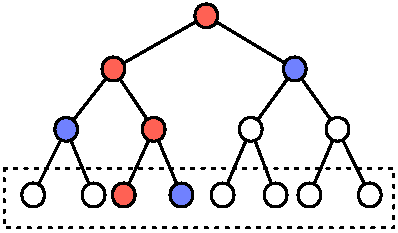
\includegraphics[width=0.2\textwidth]{hw72tree}
  \caption{Sample binary tree for 8 elements}
  \label{fig:pb2}
  \end{figure}

  \textbf{Correctness:} the correctness for getting the largest element is obvious. The reason why the $2^{nd}$ largest element can only be among the same-trace siblings (blue elements in fig \ref{fig:pb2}) is that each of the same-trace sibling is the largest in a sub tree, and all such subtrees combined make up the entire input array without the largest element. So the largest among these subtrees is the $2^{nd}$ largest in the original array.

\item[3]{Element uniqueness lower bound and closest pair}
 
  \textbf{Proof by contradiction:} assume that there's an algorithm $S$ for unbounded closest pairs that's $o(n \log n)$. We can then build an $o(n \log n)$ unbounded Element Uniqueness algorithm in the following way:

  Consider an input of $n$ elements $x_1...x_n$ for the unbounded Element Uniqueness problem, run $S$ on the pairs $(x_1, x_1), ..., (x_n, x_n)$ takes $o (n \log n)$, and gives back pairs $(x_i, x_i), (x_j, x_j)$ as being closest. Then we calculate the distance between $(x_i, x_i)$ and $(x_j, x_j)$, if 0, not all elements in $x_1...x_n$ are distinct; otherwise all elements in $x_1...x_n$ are distinct. And we've an $o(n \log n)$ unbounded Element Uniqueness algorithm.

  This contradicts with the given conclusion that unbounded Element Uniqueness is at least $O(n \log n)$, thus there's no algorithm for unbounded closest pair that's $o(n \log n)$.

\item[4]{Convex hull divide and conquer}

  The algorithm's given in alg \ref{alg:convex-hull-divide and conquer}, and is initiated by calling $convex($set of points$)$. The idea's that we first sort the points by their X-axis, and divide them into two groups with about the same number of points in each. If either group has less than 4 points, we just connect all the points in the group. Otherwise, we call divide recursively (line \ref{line:start1} - \ref{line:end1}).

  Now assume that we have the convex hull of both the left and the right group, we want to merge the two by finding the top and bottom tangents\footnote{A tangent is a line connecting a point in the left group and a point in the right group, and crosses both the left and right convex hulls exactly once} for both groups and discarding all points whose X-axis value falls in between. We find the tangents by starting with a line between $p_r$, the leftmost point in the right group, and $p_l$, the rightmost point in the left group. To find the lower tangent (line \ref{line:start2} - \ref{line:end2}), we check if $p_r$'s counter-clockwise neighbor is below this line, if so, we drop $p_r$ and move $p_r$ to its counter-clockwise neighbor. Similarly, we check and move $p_l$ clockwise. Finding the upper tangent (line \ref{line:start3} - \ref{line:end3}) is symmetric with the lower tangent.

  With the tangents added and nodes in between dropped, we then return the remaining nodes in $P$ in order, and we have a convex hull for the left and right groups combined.

  \begin{algorithm}[H]
  \caption{Convex hull divide and conquer}
  \label{alg:convex-hull-divide and conquer}
    \begin{algorithmic}[1]
    
    \Function{convex}{P}
      \State $convexHull(P.sortByX())$
    \EndFunction

    \Function{convexHull}{P}
      \State $n \gets len(P)$
      \label{line:start1}
      \If {$n \leq 3$}
        \State \Return {$connectAll(P)$}
      \EndIf
      
      \State $left \gets convexHull(P_1...P_{\frac{n}{2}})$
      \State $right \gets convexHull(P_{\frac{n}{2} + 1}...P_n)$
      \label{line:end1}

      \State $p_l \gets rightMost(left)$
      \label{line:start2}
      \State $p_r \gets leftMost(right)$
      \While {$line(p_l, p_r).isTangent(left) = false$}
        \State $discard(p_l)$
        \State $p_l \gets p_l.nextClockwise()$
      \EndWhile
      \While {$line(p_l, p_r).isTangent(right) = false$}
        \State $discard(p_r)$
        \State $p_r \gets p_r.nextCounterClockwise()$
      \EndWhile
      \State $addLine(p_l, p_r)$ 
      \label{line:end2}

      \State
      \While {...}
      \label{line:start3}
      \State ...similar with previous two loops, find upper tangent...
      \EndWhile
      \label{line:end3}
      \State

      \State \Return {those $P$ that are not discarded}

    \EndFunction

    \end{algorithmic}
  \end{algorithm}

  \textbf{Time complexity:} given the description, at worst we need to visit all $n$ nodes exactly once in a merge of $n$ nodes. During each visit, the check $isTangent$ is constant time (as we only need to check one neighbor each time). So the complexity is represented as $T(n) = 2T(\frac{n}{2}) + n$. And by master theorem (also, the same complexity representation as mergesort), the algorithm is $O(n \log n)$.

  \textbf{Correctness:} the algorithm's correctness is obvious per the description of the merging process and definition of upper / lower tangents. As an example, figure \ref{fig:pb4} illustrates the correctness of finding the lower tangent and the merging process. (left 3 and right 4 nodes are being merged. When finding the lower tangent, the lines we tried are denoted as red dotted lines, and red nodes are discarded as we try those lines. The blue dotted lines are the tangents we find eventually; and all the blue lines, along with the remaining nodes, are outputted as a convex hull).

  \begin{figure}[h]
  \centering
  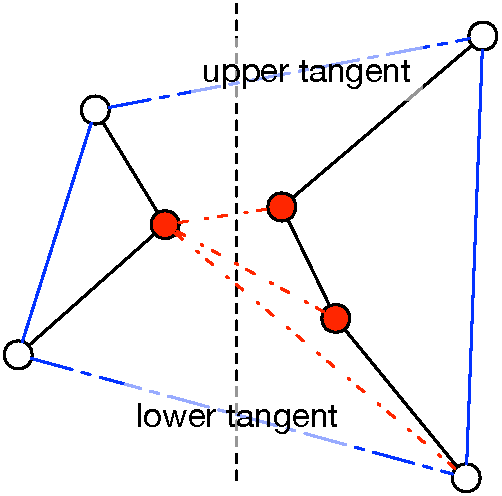
\includegraphics[width=0.2\textwidth]{hw74tangents}
  \caption{The merging process}
  \label{fig:pb4}
  \end{figure}

\end{description}

\end{document}
